\documentclass{beamer}

\usepackage[]{graphicx}
\usepackage[]{color}
%% maxwidth is the original width if it is less than linewidth
%% otherwise use linewidth (to make sure the graphics do not exceed the margin)
\makeatletter
\def\maxwidth{ %
  \ifdim\Gin@nat@width>\linewidth
    \linewidth
  \else
    \Gin@nat@width
  \fi
}
\makeatother

\definecolor{fgcolor}{rgb}{0.345, 0.345, 0.345}
\newcommand{\hlnum}[1]{\textcolor[rgb]{0.686,0.059,0.569}{#1}}%
\newcommand{\hlstr}[1]{\textcolor[rgb]{0.192,0.494,0.8}{#1}}%
\newcommand{\hlcom}[1]{\textcolor[rgb]{0.678,0.584,0.686}{\textit{#1}}}%
\newcommand{\hlopt}[1]{\textcolor[rgb]{0,0,0}{#1}}%
\newcommand{\hlstd}[1]{\textcolor[rgb]{0.345,0.345,0.345}{#1}}%
\newcommand{\hlkwa}[1]{\textcolor[rgb]{0.161,0.373,0.58}{\textbf{#1}}}%
\newcommand{\hlkwb}[1]{\textcolor[rgb]{0.69,0.353,0.396}{#1}}%
\newcommand{\hlkwc}[1]{\textcolor[rgb]{0.333,0.667,0.333}{#1}}%
\newcommand{\hlkwd}[1]{\textcolor[rgb]{0.737,0.353,0.396}{\textbf{#1}}}%

\usepackage{framed}
\makeatletter
\newenvironment{kframe}{%
 \def\at@end@of@kframe{}%
 \ifinner\ifhmode%
  \def\at@end@of@kframe{\end{minipage}}%
  \begin{minipage}{\columnwidth}%
 \fi\fi%
 \def\FrameCommand##1{\hskip\@totalleftmargin \hskip-\fboxsep
 \colorbox{shadecolor}{##1}\hskip-\fboxsep
     % There is no \\@totalrightmargin, so:
     \hskip-\linewidth \hskip-\@totalleftmargin \hskip\columnwidth}%
 \MakeFramed {\advance\hsize-\width
   \@totalleftmargin\z@ \linewidth\hsize
   \@setminipage}}%
 {\par\unskip\endMakeFramed%
 \at@end@of@kframe}
\makeatother

\definecolor{shadecolor}{rgb}{.97, .97, .97}
\definecolor{messagecolor}{rgb}{0, 0, 0}
\definecolor{warningcolor}{rgb}{1, 0, 1}
\definecolor{errorcolor}{rgb}{1, 0, 0}
\newenvironment{knitrout}{}{} % an empty environment to be redefined in TeX

\usepackage{alltt}
\mode<presentation>
{
  \usetheme{Madrid}      % or try Darmstadt, Madrid, Warsaw, ...
  \usecolortheme{beaver} % or try albatross, beaver, crane, ...
  \usefonttheme{serif}  % or try serif, structurebold, ...
  \setbeamertemplate{navigation symbols}{}
  \setbeamertemplate{caption}[numbered]
} 
\usepackage{bm} %to add math symbol@?}
\usepackage{graphicx} %to include graphics%
\usepackage{longtable}
\usepackage{lscape}
\usepackage{float}
\usepackage{epsfig} % to include EPS figure
\usepackage{epstopdf} % to include EPS figure
\usepackage{ragged2e}
\usepackage{tabularx,booktabs} %to make table
\usepackage{ragged2e}
\usepackage{tikz}
\usetikzlibrary{arrows,positioning}
\usepackage{amsmath} %this is for equation
\usepackage{breqn} %this also for equation
\usepackage[english]{babel}
\usepackage[utf8x]{inputenc}
\usepackage{xcolor}
\usepackage{listings}
\usepackage[group-separator={,}]{siunitx}
\lstset
{
    language=[LaTeX]TeX,
    breaklines=true,
    basicstyle=\tt\scriptsize,
    %commentstyle=\color{green}
    keywordstyle=\color{blue},
    %stringstyle=\color{black}
    identifierstyle=\color{magenta},
}

\title[RCT Findings]{Speaking Truth to Twitter}
\author{Team 3}
\institute[HSOG]{Hertie School of Governance}
\date{May 12, 2016}

\AtBeginSection[]
{
  \begin{frame}<beamer>
    \frametitle{Outline}
    \tableofcontents[currentsection,currentsubsection]
  \end{frame}
}
\IfFileExists{upquote.sty}{\usepackage{upquote}}{}
\begin{document}

\begin{frame}
  \titlepage
\end{frame}

\begin{frame}{Outline}
  \tableofcontents
\end{frame}





%----------Beginning of Slides----------%

\section{Implementation}
\begin{frame} {Main changes}
	\begin{itemize}
	\item We only focussed on Trump, not Clinton
	\item Our sample was drawn from unconnected accounts which had recently liked a Trump tweet (4420)
	\item We randomly assigned 1000 accounts to our treatment group and 3420 to our control group
	\end{itemize}
\end{frame}

\begin{frame}{Implementation}
	\begin{itemize}
	\item We created \num{5} similar Twitter accounts % with same 	profile picture and information but different names 
	(\textbf{@twi\_truth, @truth\_to\_twitt, @truthToTwitt, @SpeakingTw, @facts\_for\_twitt}) - see figure  \ref{fig:twit_prof}
	\item We regularly created Twitter Apps for each account. Robots used these to automatically tweet the treatment groups
	\item We sent nearly \num{7000} tweets over \num{19} days (see table \ref{table:example_tweets})
	\item Our server automatically monitored our observation group, recording \num{1475347} tweets and \num{170516} likes
	\end{itemize}
\end{frame}

\begin{frame}{Implementation}
		\begin{figure}
			\begin{centering}
  	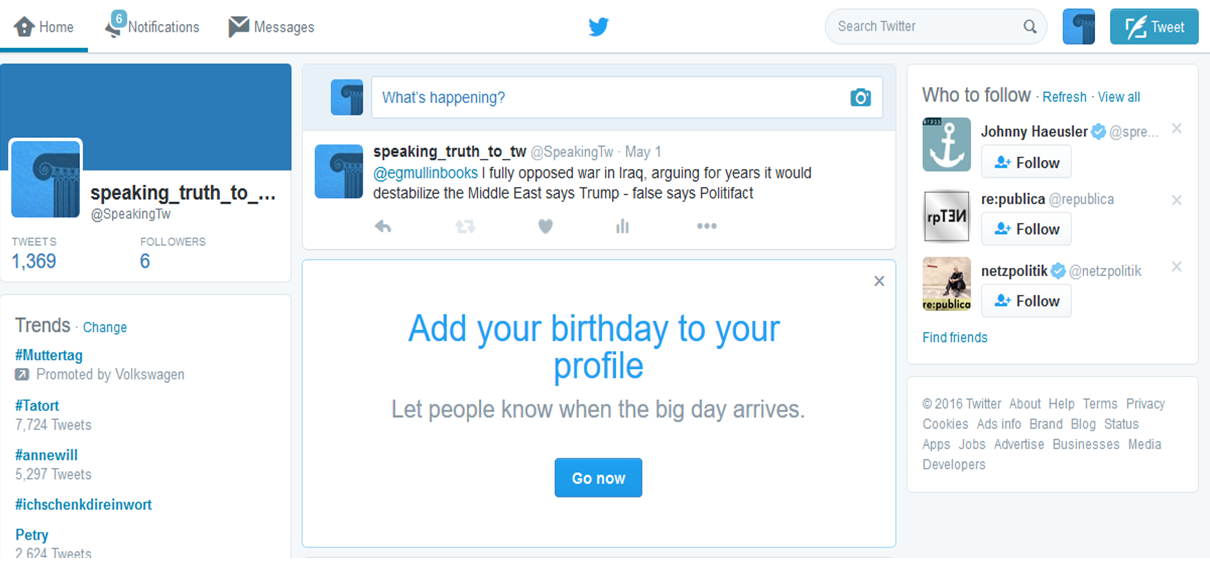
\includegraphics[scale=.45]{twitter_page.PNG}
  \caption{Example Twitter profile}
  \label{fig:twit_prof}
			\end{centering}
		\end{figure}
\end{frame}


\begin{frame}{Implementation}
\begin{table}
		\begin{center}
	{\raggedleft\tiny
	\begin{table}[ht]
\centering
\begin{tabular}{cp{6cm}cc}
  \hline
Tweet number & Text & Truth & Start date \\ 
  \hline
  1 & @LostinMemphis Trump says most wire transfers to Mexico from undocumented immigrants- half true says award-winning website Politifact &   0 & 2016-04-14 \\ 
    2 & @LostinMemphis Trump says his deficit to Clinton much smaller than Reagan's against Carter- false says award-winning website Politifact &  -2 & 2016-04-20 \\ 
    3 & @LostinMemphis Trump says Ted Cruz is mathematically out of winning the race - mostly true says politifact &   1 & 2016-04-22 \\ 
    4 & @LostinMemphis Trump says PA lost 35\%, and Harrisburg 40\%, of manufacturing jobs since 2001 - Mostly true says politifact &   1 & 2016-04-25 \\ 
    5 & @LostinMemphis Trump says football coach Rex Ryan won championships in NY twice - false says Politifact. He never did &  -2 & 2016-04-27 \\ 
    6 & @LostinMemphis Trump says ISIS makes millions of dollars a week by selling Libyan oil - false says Politifact &  -2 & 2016-04-29 \\ 
    7 & @LostinMemphis Trump says he fully opposed war in Iraq arguing for years it would destabilize the Middle East - false says Politifact &  -2 & 2016-04-30 \\ 
   \hline
\end{tabular}
\caption{Example tweets} 
\label{table:example_tweets}
\end{table}

	}
	\end{center}
\end{table}	

%\item how many tweets (+ maybe list of the tweets)
%\item graph showing when the tweets were sent over the sample period 
%\item some information on the level of (unexpected) engagement of our treatment group with us (number of retweets and likes of our tweets, number of followers, number and examples of replies to our tweets)
\end{frame}


\section{Descriptive Statistics}
\begin{frame}{Descriptive Statistics}


\begin{figure}
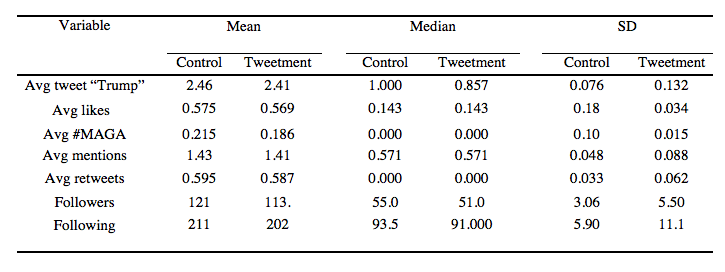
\includegraphics[width=10cm]{../tables/descriptive.png}
\end{figure}

% 	Information on our sample: table comparing the treatment and the control group containing for example the following things:
% 
% 	\begin{itemize}
% \item size of both groups (n)
% \item twitter activity (likes\_n, tweets\_n) before the experiment
% \item number of friends and/or followers
% \item male/female (do we have that information?)
% 	\end{itemize}
\end{frame}
%-----------------------------------------------%


\begin{frame}{Descriptive Statistics}

\begin{figure}
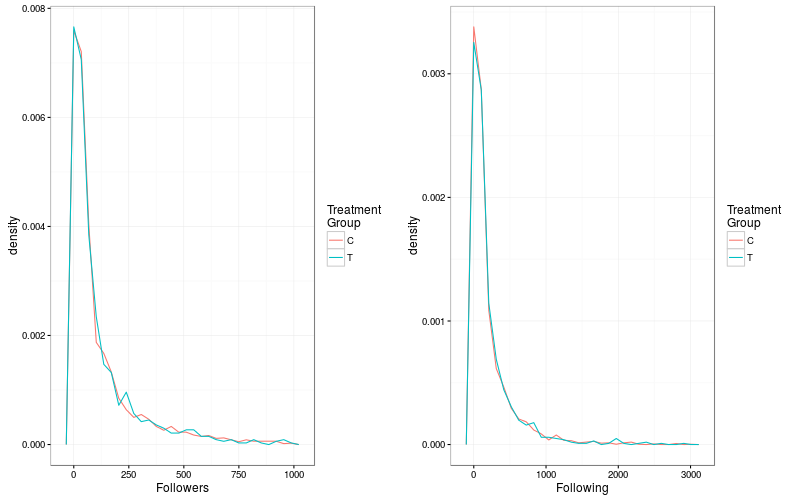
\includegraphics[width=11cm]{../plots/hists.png}
\end{figure}

\end{frame}


\section{Results}
\begin{frame}{Results: Data and Dependent Variables}
From the like and tweet data we collected, we used the following as dependent variables (all per user per day) - tweet data excludes replies to our tweets

\begin{itemize}
\item number of likes of tweets by Donald Trump
\item number of retweets of tweets by Donald Trump
\item number of tweets using the hashtag ``\#MakeAmericaGreatAgain''
\item number of tweets including the key word ``Trump''
\end{itemize} 
\end{frame}

\section{Results}
\begin{frame}{Results: Data and Dependent Variables}

\begin{figure}
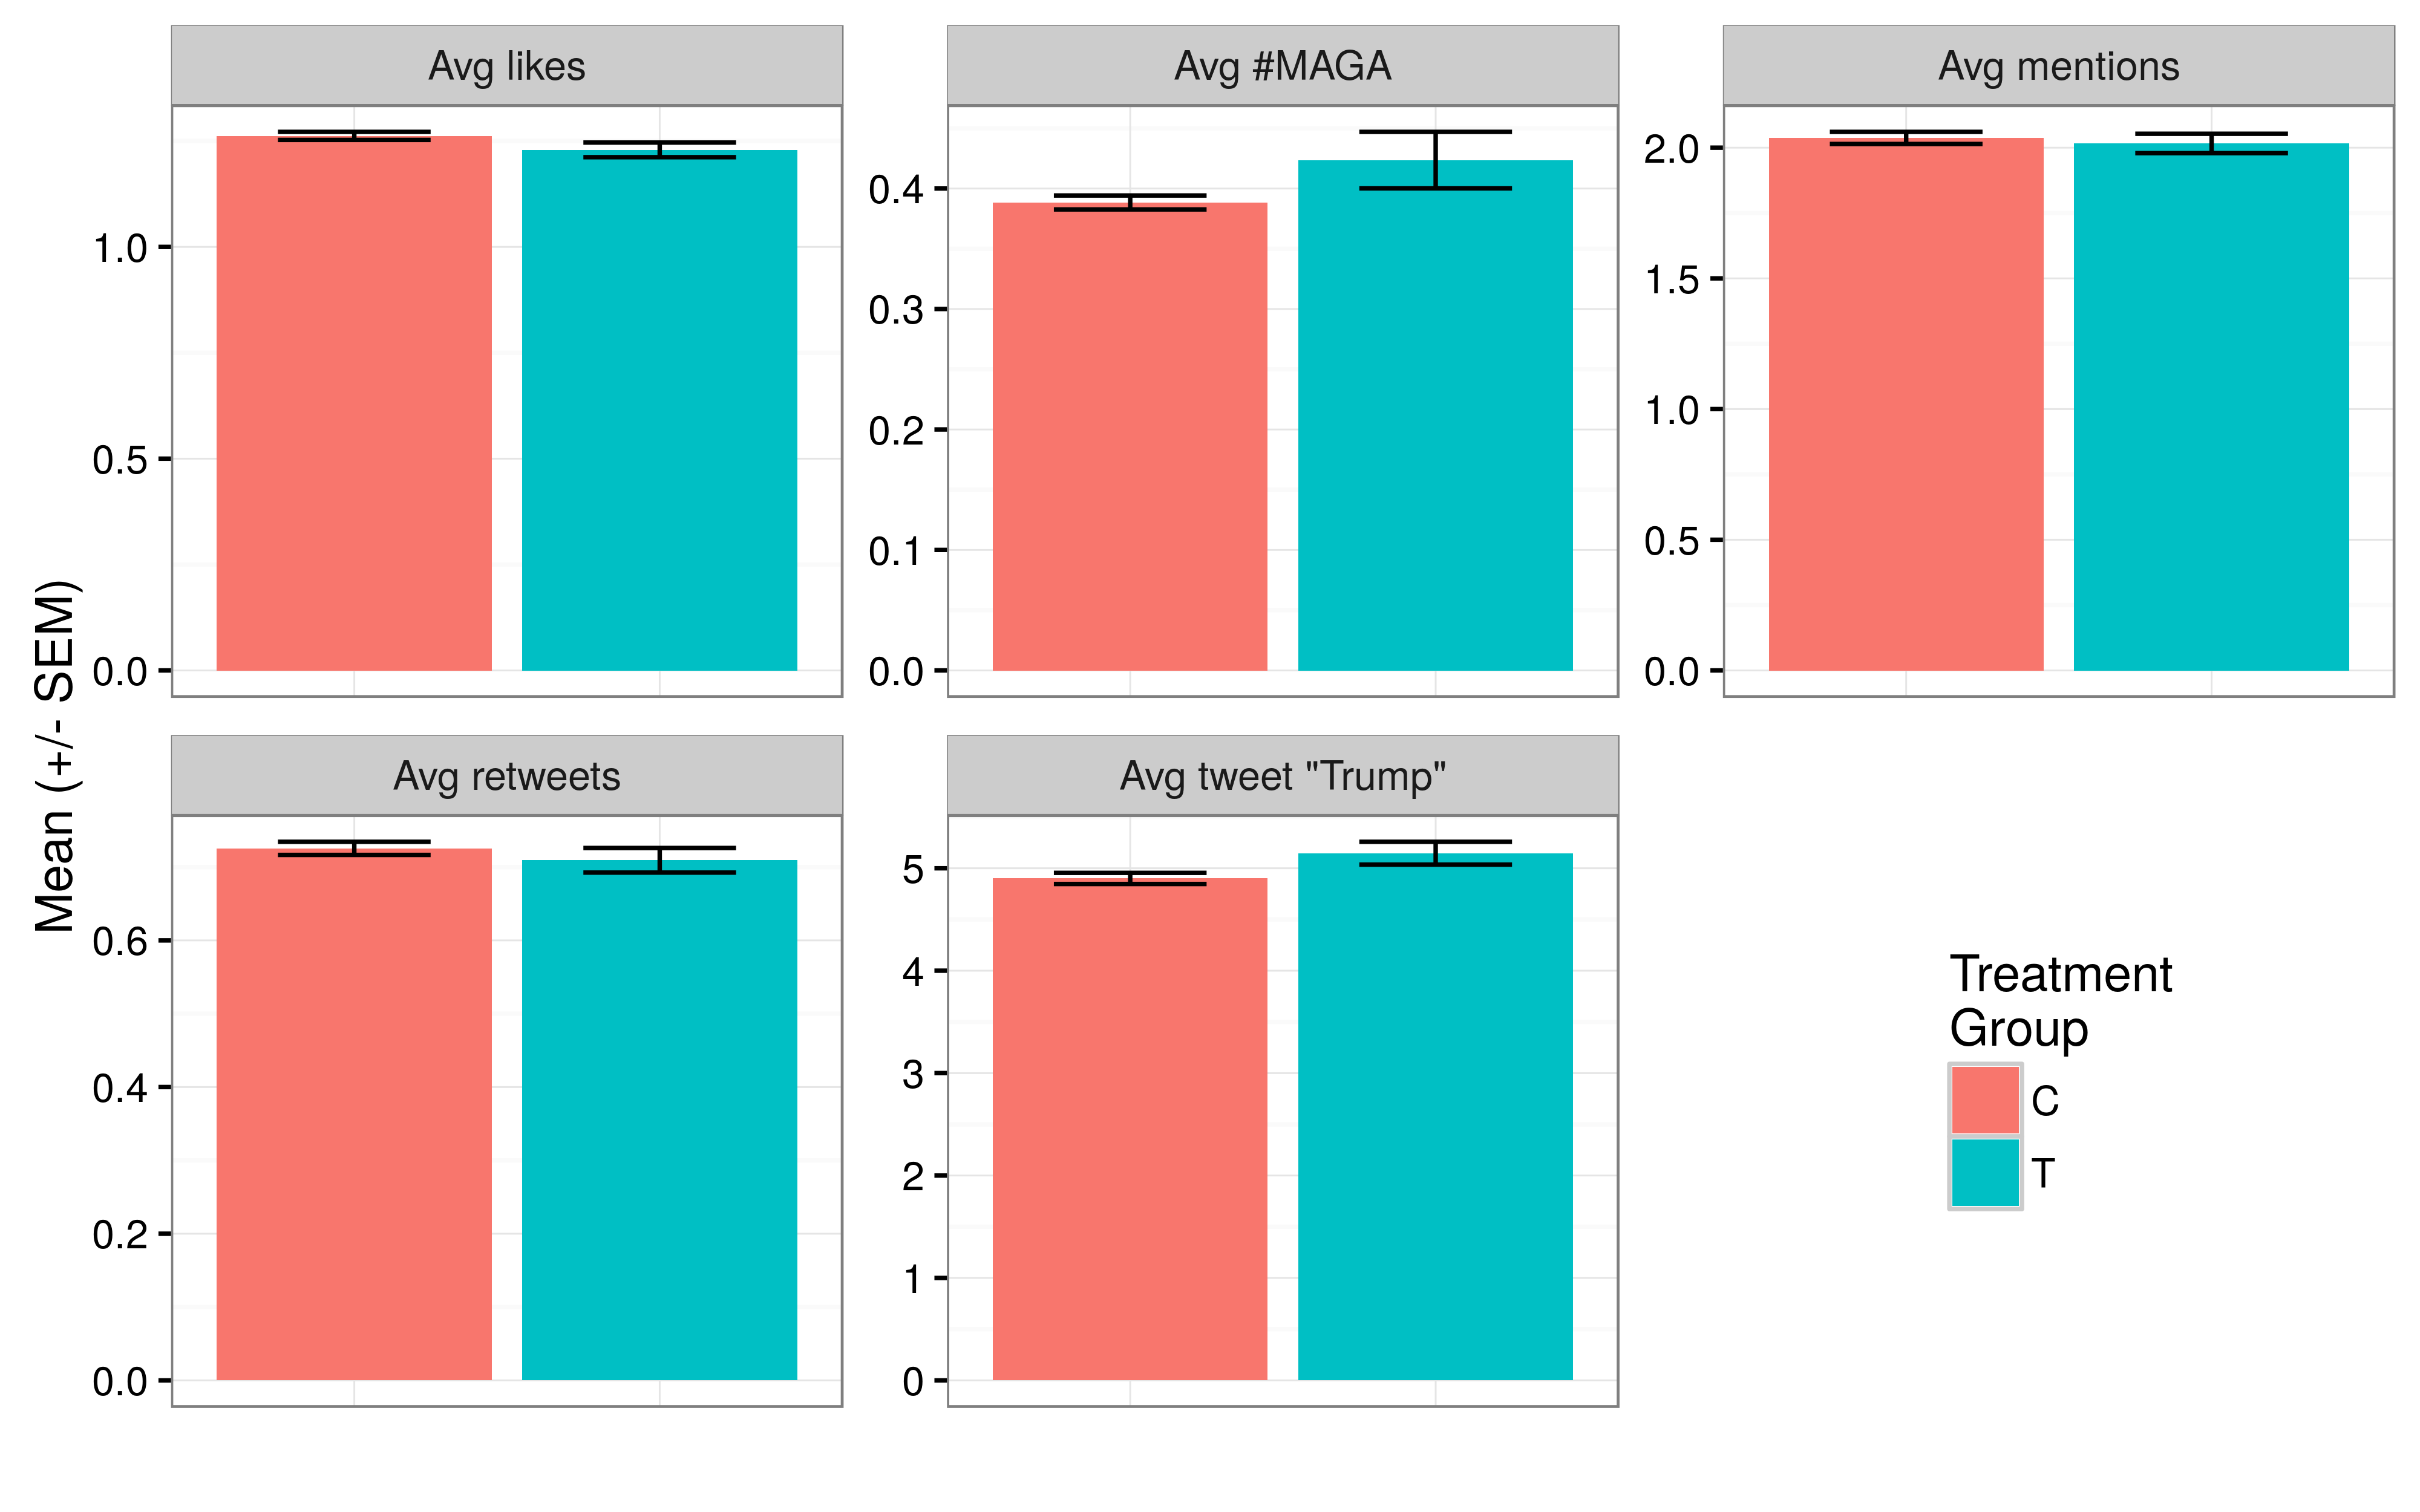
\includegraphics[width=9cm]{../plots/mean_bars.png}
\label{fig:mean_bars}
\caption{Per user per day means of each dependent variable in treatment and control groups during the treatment period}
\end{figure}




\end{frame}


\section{Limitations}
\begin{frame}{Limitations}
\begin{itemize}

\item Self selection in the sample: 
\textit{Only active trump followers were selected in our study} and \textit{People had the option to opt-out}
	\item 10 individuals asked to be withdrawn during treatment. Effect measured thus ITT effect
\item Being recognized as a robot
\item Bias from manipulation of the twitter feed
\item Outcome is \textbf{likes} or \textbf{tweets} per day while the tweeting has been done at a certain time during the day...
\item Collinearity of variables in case of the lasting turn-on model!
\end{itemize}
\end{frame}




\begin{frame}{Interesting}
		\begin{figure}
			\begin{centering}
  	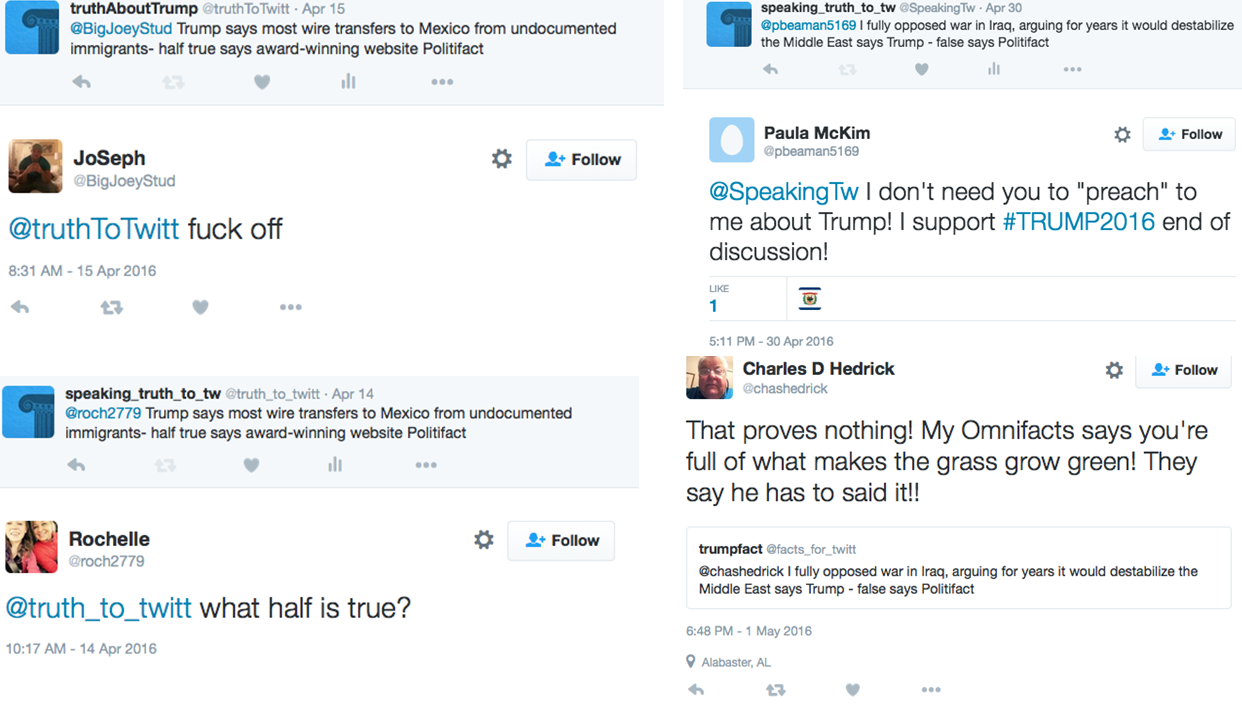
\includegraphics[scale=.45]{twitter_comment.PNG}
  \caption{Some interesting comments}
			\end{centering}
		\end{figure}
\end{frame}
		
\end{document}
